\newpage
\section{Vorbereitung}
Machen Sie Sich vertraut mit der Bibliothek Serial unter \url{http://energia.nu/reference/serial} und \url{http://energia.nu/Tutorial\_SerialEvent.html}. Und lesen Sie \url{http://energia.nu/guide/tutorial\_tone/}.\\
\begin{figure}[h]
\centering
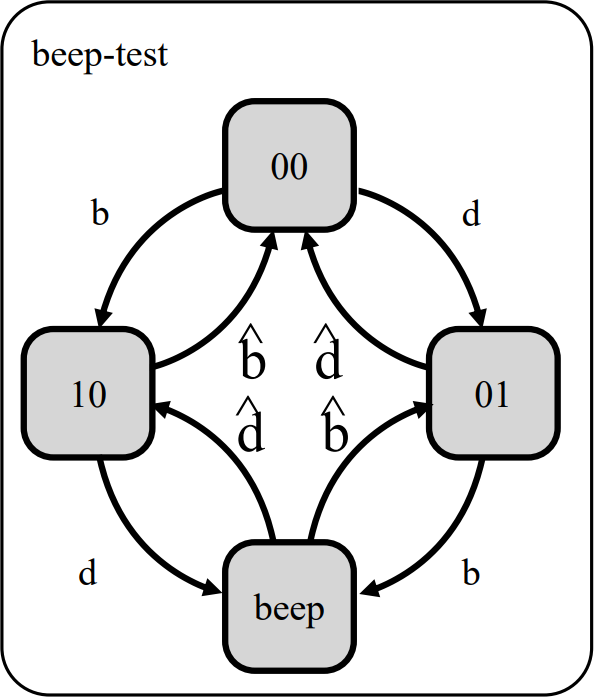
\includegraphics[width=0.3\linewidth]{images/beep-test}
\caption{Zustandsmaschine $"$beep-test$"$}
\label{fig:beep-test}
\end{figure}

\noindent In der Vorlesung wurde über die Zustandsmaschine $"$beep-test$"$ im Rahmen eines Statecharts zu einer Digitaluhr gesprochen. Diese Zustandsmaschine ist in Abbildung 1 gezeigt.\\ \\
Schlie\ss{}en Sie das LaunchPad an das Steckbrett gemä\ss{} dem Schaltbild 2 an. Die Ereignisse b, d, \^b, \^d sollen durch die Schaltknöpfe generiert werden. Die Ausgabe eines Tons soll über den Piezo-Buzzer erfolgen. Die Schaltknöpfe sind über die Pins PC4 und PC5, der Piezo-Buzzer über den Pin PC6 anzuschlie\ss{}en.\\
\begin{figure}[h]
\centering
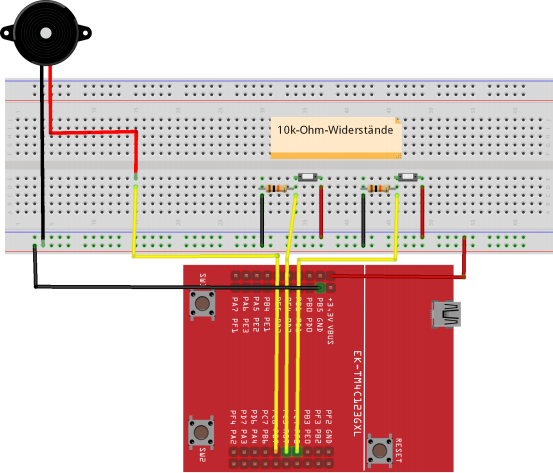
\includegraphics[width=0.5\linewidth]{images/Schaltbild2}
\label{fig:Schaltblid2}
\end{figure}
\begin{center}
	Schaltbild 2
\end{center}
\newpage
\section{Aufgabe 1}
Implementieren Sie auf dem Board die Zustandsmaschine aus Abbildung 1.\\
\section{Aufgabe 2}
Verwenden Sie die Schaltung gemä\ss{} dem Schaltbild 2 für einen Morsecode-Übersetzer. Eine Morsecode-Tabelle finden Sie auf Wikipedia unter \url{http://de.wikipedia.org/wiki/Morsecode}.\\ \\
Programmieren Sie auf dem Board einen Morsecode-Übersetzer. Das Programm soll folgende Eigenschaften erfüllen:\\
\begin{itemize}
	\item Empfangen eines ASCII-Textes über die serielle Verbindung vom Rechner, an dem das LaunchPad angeschlossen ist. Stellen Sie sicher, dass die Länge des Textes 128 Bytes nicht überschreitet.
	\item Übersetzen des ASCII-Textes in einen Morsecode, der über den Piezo-Buzzer oder über die LED des Boards ausgegeben werden kann. Mit dem Knopf an Pin PC4 muss zwischen den beiden Ausgabemöglichkeiten gewählt werden können. Gestalten Sie das Programm mittels Objektorientierung und Polymorphie flexibel, so dass für beide Ausgaben das gleiche Interface verwendet wird.
	\item Der Morsecode muss jeweils einmal ausgegeben werden, wenn der Knopf an Pin PC5 bestätigt wird. Dabei soll die Zeichenkette gespeichert werden, so dass keine Neueingabe vor Ausgabe des Morsecodes notwendig ist.
\end{itemize}
